\subsection{Question 1}
 Le protocole peut être décrit par le réseau suivant : \\

\begin{figure}[H]
  \centering
  \begin{tikzpicture}

    % Liste des places
    \draw (-6,2) node[below right = 2pt] {$P_1$};
    \node[draw,circle,scale=2] (P1) at (-6, 2) {};
    \draw (-2,2) node[below right = 2pt] {$P_2$};
    \node[draw,circle,scale=2] (P2) at (-2, 2) {};
    \draw (-4,0) node[below right = 2pt] {$P_3$};
    \node[draw,circle,scale=2] (P3) at (-4,0) {};
    \draw (2,2) node[below right = 2pt] {$P_4$};
    \node[draw,circle,scale=2] (P4) at (2, 2) {}; %%
    \draw (0,0) node[below right = 2pt] {$P_5$}; 
    \node[draw,circle,scale=2] (P5) at (0,0) {};
    \draw (2,-2) node[below left = 2pt] {$P_6$};
    \node[draw,circle,scale=2] (P6) at (2, -2) {};

    % Liste des transitions
    \draw (-4,2) node[below = 10pt] {$t_1$};
    \node[draw,rectangle,yscale=4] (t1) at (-4, 2) {};
    \draw (2,0) node[below = 10pt] {$t_3$};
    \node[draw,rectangle,yscale=4] (t3) at (2, 0) {};
    \draw (0,2) node[below = 10pt] {$t_2$};
    \node[draw,rectangle,yscale=4] (t2) at (0, 2) {};
    \draw (-6,-0) node[below = 10pt] {$t_5$};
    \node[draw,rectangle,yscale=4] (t5) at (-6, 0) {};
    \draw (4,2) node[below = 10pt] {$t_4$};
    \node[draw,rectangle,yscale=4] (t4) at (4, 2) {};
    
        % Liste des arcs
    \draw[->,>=latex] (P1) -- (t1);
    \draw[->,>=latex] (t1) -- (P3);
    \draw[->,>=latex] (P3) -- (t5);
    \draw[->,>=latex] (t5) -- (P1);
    \draw[->,>=latex] (t1) -- (P2);
    \draw[->,>=latex] (P2) -- (t5);
    \draw[->,>=latex] (P2) -- (t2);
    \draw[->,>=latex] (P5) -- (t2);
    \draw[->,>=latex] (t2) -- (P4);
    \draw[->,>=latex] (P4) -- (t3);
    \draw[->,>=latex] (t3) -- (P6);
    \draw[->,>=latex] (P6) -- (t4);
    \draw[->,>=latex] (P4) -- (t4);
    \draw[->,>=latex] (t4) -- (P5);
    \draw[->,>=latex] (t4) to [out=90,in=90] (P1);

    % Marquage 
    \draw [fill](-6,2) circle (0.1) ;
    \draw [fill](0,0) circle (0.1) ;
  \end{tikzpicture}
  \caption{Réseau de petri associé à l'exercice 5} \label{fig:M5}
\end{figure}

Quand l'utilisateur rentre en communication,l'attente du controleur est symbolisé par le faite qu'il n'y est pas de jeton dans celui-ci.

\begin{center}

{\Huge C}\qquad =\qquad $\bordermatrix{
&t_1&t_2&t_3&t_4&t_5&\cr
P_1&-1&0&0&-1&1\cr
P_2&1&-1&0&0&-1\cr
P_3&1&0&0&0&-1\cr
P_4&0&1&-1&-1&0\cr
P_5&0&-1&0&1&0\cr
P_6&0&0&1&-1&0\cr
}$

\end{center}

\subsection{Question 2}
Soit $f=(f_1\ f_2\ f_3\ f_4\ f_5\ f_6)$ le vecteur générique de P-flots.\\
On cherche : 
\begin{center}
$\begin{pmatrix}
-1 & 0 & 0 & -1 & 1\\
 1 & -1 & 0 & 0 & -1\\
 1 & 0 & 0 & 0 & -1\\
 0 & 1 & -1 & -1 & 0\\
 0 & -1 & 0 & 1 & 0\\ 
 0 & 0 & 1 & -1 & 0\\
\end{pmatrix}
\begin{pmatrix}
f_1\\
f_2\\ 
f_3\\ 
f_4\\ 
f_5\\ 
f_6
\end{pmatrix}
=0
$

\vspace{0.5cm}

$\rightarrow 
\begin{cases}
-f_1 + f_2 + f_3 = 0\\
f_2 + f_4 - f_5  = 0\\
-f_4 + f_6  = 0\\
-f_1 - f_4 + f_5 - f_6 = 0
\end{cases}$

\vspace{0.5cm}
On trouve donc 2 P-Flots :\\
$
f_1 = 1 \ (1 \ -1 \ \ 0 \ \ 0 \ \ 1 \ \ 0)
$
\\
$
f_4 = 1 \ (0 \ -1 \ -3 \ 1 \ 2 \ 1)
$

\end{center}
\subsection{Question 3}
Soit $f=(f_1\ f_2\ f_3\ f_4\ f_5\ f_6)$ le vecteur générique de P-semiFlots.\\
\begin{center}
Le calcul a été réalisé avec Tina , on trouve 2 P-semiFlots: \\
$f_1 = (2\ 1\ 1\ 1\ 0\ 1)$\\
$f_2 = (1\ 0\ 1\ 1\ 1\ 1)$

\vspace{0.5cm}

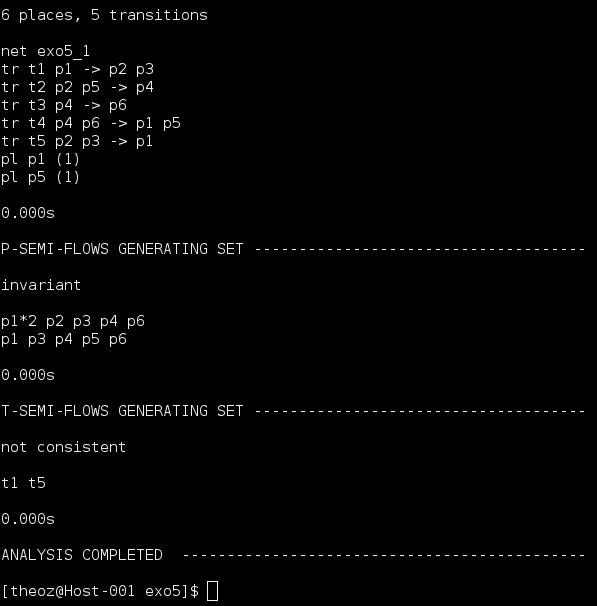
\includegraphics[width=0.35\textwidth]{images/screenTinaExo5.png}\\
\end{center}